%%%%%%%%%%%%%%%%%%%%%%%%%%%%%%%%%%%%%%%%%%%%%%%%%%%%%%%%%%%%%%%%%%%%%%%%%%%%%%%%
% > Лабораторная работа 4: Крутильные колебания вала с дисками.
% > Баталов Семен, Антонова Мария, Клюшин Максим, Хайретдинова Диана.
% > 2021 год.
%%%%%%%%%%%%%%%%%%%%%%%%%%%%%%%%%%%%%%%%%%%%%%%%%%%%%%%%%%%%%%%%%%%%%%%%%%%%%%%%

\documentclass[12pt, a4paper]{article}
\usepackage[left=2cm, right=2cm, top=2.5cm, bottom=2.5cm, nohead, 
footskip=1cm]{geometry}
\usepackage{graphicx}
\graphicspath{{./Pictures/}}
\usepackage[utf8]{inputenc}
\usepackage[english, russian]{babel}
\usepackage{indentfirst}
\usepackage{array}
\usepackage{longtable}
\usepackage{misccorr}
\usepackage{setspace, amsmath}
\usepackage{multirow}

\begin{document}
    
    \newcolumntype{M}[1]{>{\centering\arraybackslash}m{#1}}
    \renewcommand{\arraystretch}{1.4}
    
    \begin{center}
        \large{Санкт-Петербургский государственный университет} \\
        \large{Saint-Petersburg State University}\\
        \hfill \break
        \hfill \break
        \hfill \break
        \hfill \break
        \hfill \break
        \hfill \break
        \hfill \break
        \large{Кафедра теоретической и прикладной механики} \\
        \hfill \break
        \hfill \break
        \large{\textbf{ОТЧЕТ}} \\
        \large{\textbf{По лабораторной работе 4}} \\
        \large{<<Крутильные колебания вала с дисками>>} \\
        \hfill \break
        \hfill \break
        \hfill \break
        \large{По дисциплине} \\
        \large{<<Лабораторный практикум по теоретической механике>>} \\
    \end{center}
    
    \hfill \break
    \hfill \break
    \hfill \break
    \hfill \break
    \hfill \break
    \hfill \break
    
    \begin{flushright} 
        \large{Выполнили:} \\
        \hfill \break
        \large{Баталов С. А.} \\
        \large{Антонова М. } \\
        \large{Клюшин М.} \\
        \large{Хайретдинова Д.} \\
    \end{flushright}
    
    \hfill \break
    \hfill \break
    \hfill \break
    \hfill \break
    
    \begin{center} 
        \large{Санкт-Петербург} \\
        \large{2021} \\
    \end{center}
    
    \thispagestyle{empty}
    \newpage
    
    \section{Описание установки}
    
    В данной работе рассматриваются колебания механической системы с тремя степенями свободы. Целью работы является экспериментальное определение частот и главных форм собственных колебаний системы, их теоретический расчет и последующее сравнение.
    
    \begin{figure} [h]
        \centering
        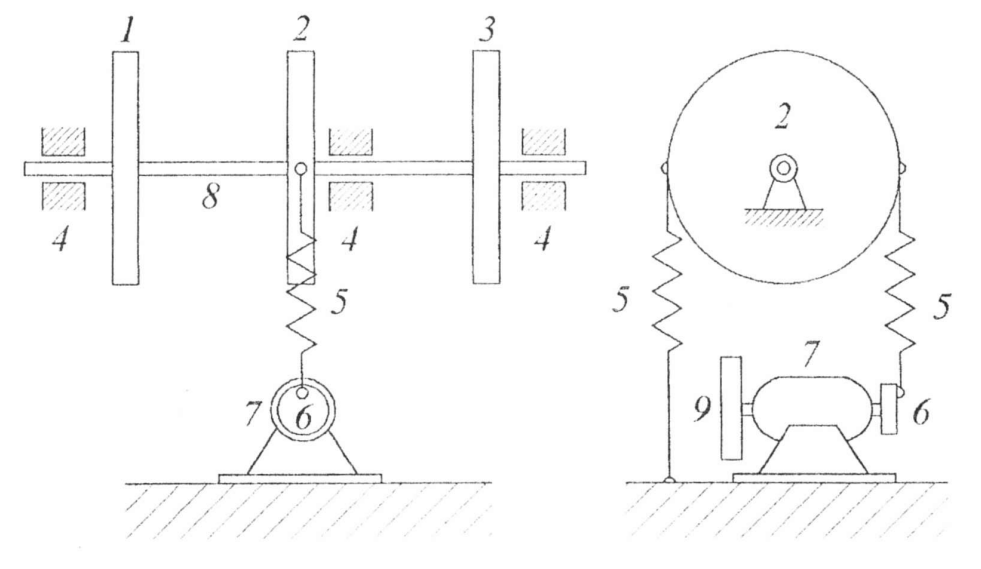
\includegraphics [width = 12cm] {Lab_4_1.png}
        \caption{\centering Схема лабораторной установки.}
        \label{im1}
    \end{figure}
    
    На рис.~\ref{im1} изображена схема лабораторной установки. Основной частью установки является упругий вал \textit{8} с тремя жестко укрепленными на нем дисками \textit{1}, \textit{2} и \textit{3}. Вал может вращаться в подшипниках \textit{4}, установленных на станине. К ободу среднего диска \textit{2} прикреплены пружины \textit{5}, одна из которых связана со станиной, а другая~--~с эксцентриком \textit{6}, закрепленном на валу электродвигателя \textit{7}. На валу электродвигателя укреплены маховик \textit{9} для стабилизации частоты вращения и диск оптоэлектронного тахометрического датчика. Сигнал с тахометрического датчика поступает на вход электронного цифрового тахометра, показания которого соответствуют частоте вращения вала в герцах.
    
    \newpage
    
    \section{Параметры установки}
    
    В следующей таблице представлены заранее известные величины: плотность материала дисков~--~$\rho$, модуль сдвига материала вала~--~$G$, жесткость пружины~--~$c_{\text{п}}$.
    
    \begin{longtable}{| M{2cm} | M{3cm} | M{3cm} | M{3cm} |}
        \caption{\centering Известные константы.}
        \label{tb1} \\
        \hline
        Номер & Величина & Значение & Размерность \\
        \hline
        1 & $\rho$ & $7,85 \cdot 10^{3}$ & $\text{кг} / \text{м}^{3}$ \\
        2 & $G$ & $8,33 \cdot 10^{10}$ & Па \\
        3 & $c_{\text{п}}$ & 4900 & $\text{Н} / \text{м}$ \\
        \hline
    \end{longtable}
    
    Для расчета частот и форм собственных колебаний системы потребуется измерить некоторые параметры установки. Данные измерений приведены в таблице \ref{tb2}. Здесь $R_{i}$~--~радиусы дисков, $d_{i}$~--~толщины дисков, $l_{i}$~--~расстояния между дисками, $r$~--~радиус упругого вала, $e$~--~расстояние от точки крепления пружины до центра эксцентрика.
    
    \begin{longtable}{| M{2cm} | M{3cm} | M{3cm} | M{3cm} | M{3cm} |}
        \caption{\centering Результаты измерений параметров установки.}
        \label{tb2} \\
        \hline
        Номер & Величина & Значение & Погрешность & Размерность \\
        \hline
        1 & $R_{1}$ & 150 & 0.5 & мм \\
        2 & $R_{2}$ & 150 & 0.5 & мм \\
        3 & $R_{3}$ & 150 & 0.5 & мм \\
        \hline
        4 & $d_{1}$ & 25 & 0.5 & мм \\
        5 & $d_{2}$ & 20 & 0.5 & мм \\
        6 & $d_{3}$ & 25 & 0.5 & мм \\
        \hline
        7 & $l_{1}$ & 445 & 0.5 & мм \\
        8 & $l_{2}$ & 616 & 0.5 & мм \\
        \hline
        9 & $r$ & 5 & 0.05 & мм \\
        \hline
        10 & $e$ & ? & 0.5 & мм \\
        \hline
    \end{longtable}
    
    \newpage
    
    \section{Теоретический расчет}
    
    
    
    \newpage
    
\end{document}